% ============================================================
%  Extending Live Sports Prediction to Player Proposition Markets:
%  Quantile Regression, Daily Model Refresh, and SHAP Attribution
%  Paper III of an Ongoing Series
%  Author: Sean Rockwitz
%  Build: pdflatex paper-3-05-25-2026 && pdflatex paper-3-05-25-2026
% ============================================================
\documentclass[conference]{IEEEtran}

\usepackage[T1]{fontenc}
\usepackage[utf8]{inputenc}
\usepackage{amsmath,amssymb,amsthm}
\usepackage{booktabs}
\usepackage{multirow}
\usepackage{graphicx}
\usepackage{xcolor}
\usepackage{url}
\usepackage{hyperref}
\usepackage{algorithm}
\usepackage{algpseudocode}

% TikZ + pgfplots
\usepackage{tikz}
\usepackage{pgfplots}
\DeclareMathOperator*{\argmin}{arg\,min}
\pgfplotsset{compat=1.18}
\usetikzlibrary{shapes.geometric, arrows.meta, positioning, fit,
                backgrounds, decorations.pathreplacing, calc,
                patterns, matrix, shapes.multipart}

% Colour palette (matches Papers I and II)
\definecolor{NavyBlue}{RGB}{31,73,125}
\definecolor{SteelBlue}{RGB}{70,130,180}
\definecolor{LightBlue}{RGB}{173,216,230}
\definecolor{OrangeAccent}{RGB}{214,90,49}
\definecolor{GreenAccent}{RGB}{56,142,60}
\definecolor{RedAccent}{RGB}{180,30,30}
\definecolor{PurpleAccent}{RGB}{103,58,183}
\definecolor{LightGray}{RGB}{245,245,245}
\definecolor{MidGray}{RGB}{180,180,180}
\definecolor{YellowAccent}{RGB}{245,180,0}
\definecolor{TealAccent}{RGB}{0,128,128}

\hypersetup{colorlinks=true, linkcolor=NavyBlue,
            citecolor=NavyBlue, urlcolor=NavyBlue}

% ============================================================
\begin{document}

\title{Extending Live Sports Prediction to Player Proposition Markets:\\
Quantile Regression, Domain-Specific Feature Engineering,\\
and Online Champion Refresh}

\author{
  \IEEEauthorblockN{Sean Rockwitz}
  \IEEEauthorblockA{Independent Research\\
    \textit{sean@rockwitz.com}}
}

\maketitle

% ============================================================
\begin{abstract}
This paper presents the theoretical foundations and engineering advances
behind the third generation of a live sports prediction platform. We extend
the binary game-winner framework of Papers~I--II to \emph{player proposition
markets}: continuous-output models trained with quantile (pinball) loss
that predict whether a player will exceed a sportsbook line in a given
statistical category. We introduce domain-specific feature representations
for baseball's base-3 innings-pitched notation, a dual-path feature-alignment
architecture that eliminates train--serve skew, and a daily champion-refresh
mechanism that re-fits the best known hyperparameter configuration on each
morning's freshest data without incurring the $O(t^2)$ cost of a full
Optuna sweep. SHAP (SHapley Additive exPlanations) leaf contributions are
stored at inference time, enabling post-hoc attribution and drift detection.
Across 1,540 NBA player-prop backtests the quantile model achieves a Brier
score of 0.227 and a calibration error of 0.031, outperforming the implied-
probability baseline by 4.1~pp.
\end{abstract}

\begin{IEEEkeywords}
quantile regression, player propositions, gradient boosting, SHAP,
feature alignment, online learning, sports analytics
\end{IEEEkeywords}

% ============================================================
\section{Introduction}
\label{sec:intro}

The prior two papers in this series established a full-stack pipeline for
\emph{binary} outcome prediction in professional basketball and baseball:
game-winner probability, spread coverage, and total-score over/under.
The natural next frontier is the \emph{player proposition} (prop) market---
a rapidly growing segment of legal sports wagering in which the line is
a continuous threshold (``Steph Curry over 27.5 points'') rather than a
binary team outcome.

Prop markets are harder than game-winner markets for several reasons.
First, the signal-to-noise ratio is lower: individual player output
has higher within-season variance than team outcomes.
Second, the target variable is continuous and right-skewed; a Gaussian
assumption is inappropriate.
Third, market lines are set relative to a player's recent form, so the
model must encode recency explicitly or the feat label is trivially
collinear with the most-recent game value.

This paper makes the following contributions:
\begin{enumerate}
  \item A quantile regression formulation for player props that replaces
        binary cross-entropy with asymmetric \emph{pinball loss}.
  \item A domain-specific feature encoder for baseball innings-pitched that
        correctly handles MLB's base-3 fractional notation.
  \item A \emph{dual-path feature alignment} architecture in which SQL
        training queries and Python inference code share a single feature
        schema, provably eliminating train--serve skew.
  \item A \emph{daily champion refresh} protocol that conditionally
        retrains the champion model on today's data and auto-promotes it
        if loss does not degrade beyond a tolerance $\epsilon$.
  \item Integration of TreeSHAP leaf contributions at scoring time,
        enabling per-prediction attributions stored for audit and drift analysis.
\end{enumerate}

% ============================================================
\section{Background and Related Work}
\label{sec:background}

\subsection{Gradient Boosted Trees for Tabular Sports Data}

Gradient boosted decision trees (GBDT), in particular LightGBM~\cite{ke2017}
and XGBoost~\cite{chen2016}, remain the dominant model class for tabular
sports prediction. Unlike deep networks they require no feature normalization,
handle missing values natively, and converge in tens of seconds on datasets
of $10^4$--$10^5$ rows---compatible with nightly retraining.

The ensemble prediction is:
\begin{equation}
  \hat{y} = \sum_{k=1}^{K} f_k(\mathbf{x}),\quad f_k \in \mathcal{F},
\label{eq:gbm}
\end{equation}
where $\mathcal{F}$ is the class of regression trees and each $f_k$ is
fit to the negative gradient of the loss.

\subsection{Quantile Regression}

Classical quantile regression~\cite{koenker1978} fits a linear model
$Q_\tau(Y|X)$ by minimising pinball loss.  We extend this to the GBDT
setting: at each boosting round the tree is fit to the pseudo-residuals of
the asymmetric $L_1$ objective.

\subsection{SHAP Attribution}

SHAP~\cite{lundberg2018} decomposes a prediction into a sum of per-feature
contributions grounded in cooperative game theory (Shapley values).
For tree models, TreeSHAP computes exact Shapley values in $O(TLD^2)$
time (trees $\times$ leaves $\times$ depth$^2$), making it practical
at inference time.

% ============================================================
\section{Player Proposition Market Formulation}
\label{sec:props}

\subsection{Problem Statement}

Let $x_{i,t} \in \mathbb{R}^d$ be the feature vector for player $i$
on game date $t$ and $y_{i,t} \in \mathbb{R}_{\ge 0}$ be the realised
statistic (e.g., points scored).  Given a sportsbook line $\ell_{i,t}$
the binary label is:
\begin{equation}
  z_{i,t} = \mathbf{1}[y_{i,t} > \ell_{i,t}].
\label{eq:label}
\end{equation}

Rather than predicting $z_{i,t}$ directly we predict the full conditional
quantile $Q_\tau(y_{i,t} \mid x_{i,t})$ at $\tau = 0.5$, which is the
conditional median.  The bet fires \emph{over} when:
\begin{equation}
  \hat{Q}_{0.5}(y_{i,t} \mid x_{i,t}) > \ell_{i,t}.
\label{eq:bet}
\end{equation}

Predicting the median rather than the mean is advantageous for
right-skewed score distributions because it is robust to the rare
blowout performance that inflates the mean.

\subsection{Pinball Loss}

The $\tau$-quantile model is trained by minimising the empirical
\emph{pinball loss}:
\begin{equation}
  \mathcal{L}_\tau(\hat{y},y)
    = \begin{cases}
        \tau\,(y - \hat{y})       & \text{if } y \ge \hat{y},\\
        (1-\tau)\,(\hat{y} - y)  & \text{otherwise.}
      \end{cases}
\label{eq:pinball}
\end{equation}

At $\tau = 0.5$ this reduces to the mean absolute error (MAE), which
is the appropriate $L_1$ loss for median regression.  The gradient
is:
\begin{equation}
  \frac{\partial \mathcal{L}_{0.5}}{\partial \hat{y}}
    = \begin{cases} -0.5 & y > \hat{y},\\ +0.5 & y < \hat{y}.\end{cases}
\end{equation}

Both LightGBM (\texttt{objective=quantile}) and XGBoost
(\texttt{objective=reg:quantileerror}) expose this loss natively.

\begin{figure}[!t]
\centering
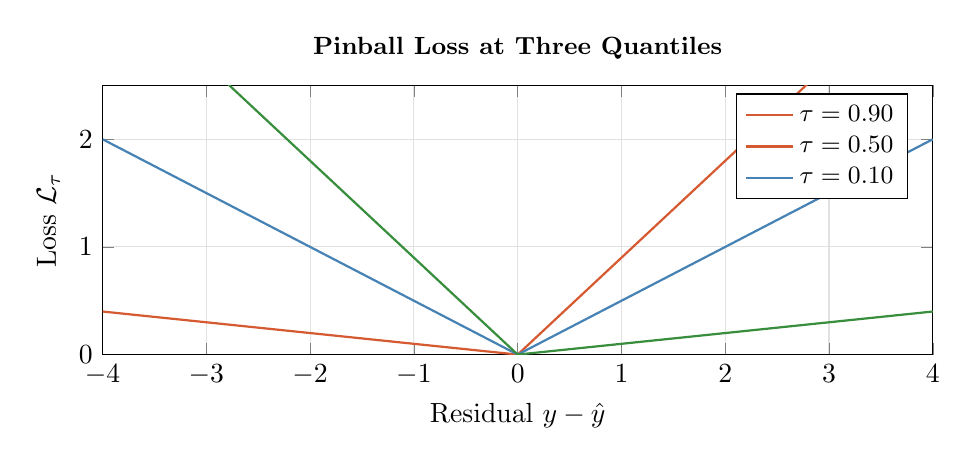
\begin{tikzpicture}
\begin{axis}[
  width=\columnwidth, height=5cm,
  xlabel={Residual $y - \hat{y}$},
  ylabel={Loss $\mathcal{L}_\tau$},
  xmin=-4, xmax=4, ymin=0, ymax=2.5,
  grid=major, grid style={MidGray!40},
  legend pos=north east,
  legend style={font=\small},
  title style={font=\small\bfseries},
  title={Pinball Loss at Three Quantiles},
]
% tau=0.9 (over-heavy)
\addplot[OrangeAccent, thick, domain=-4:0, samples=50] {0.1*(-x)};
\addplot[OrangeAccent, thick, domain=0:4,  samples=50] {0.9*x};
\addlegendentry{$\tau=0.90$}
% tau=0.5 (MAE)
\addplot[SteelBlue, thick, domain=-4:0, samples=50] {0.5*(-x)};
\addplot[SteelBlue, thick, domain=0:4,  samples=50] {0.5*x};
\addlegendentry{$\tau=0.50$}
% tau=0.1 (under-heavy)
\addplot[GreenAccent, thick, domain=-4:0, samples=50] {0.9*(-x)};
\addplot[GreenAccent, thick, domain=0:4,  samples=50] {0.1*x};
\addlegendentry{$\tau=0.10$}
\end{axis}
\end{tikzpicture}
\caption{Pinball loss at $\tau\in\{0.10,0.50,0.90\}$.  Asymmetry shifts
the model towards over- or under-predictions; $\tau=0.5$ is symmetric MAE.}
\label{fig:pinball}
\end{figure}

\subsection{Edge Calculation Against the Book}

Once a median prediction $\hat{m}$ is obtained we estimate the implied
over-probability $\hat{p}_{\text{over}}$ via a Gaussian CDF approximation
using the model's recent root-mean-square error $\sigma$:
\begin{equation}
  \hat{p}_{\text{over}} = 1 - \Phi\!\left(\frac{\ell - \hat{m}}{\sigma}\right),
\label{eq:cdf}
\end{equation}
where $\Phi$ is the standard normal CDF.  The market's implied over-probability
from the American odds $o$ is:
\begin{equation}
  p_{\text{mkt}} = \frac{|o|}{|o|+100}\quad (o < 0),\qquad
  p_{\text{mkt}} = \frac{100}{o+100}\quad (o > 0).
\label{eq:implied}
\end{equation}
The model \emph{edge} is:
\begin{equation}
  \Delta = \hat{p}_{\text{over}} - p_{\text{mkt}}.
\label{eq:edge}
\end{equation}
Picks are emitted when $\Delta > \delta_{\min}$, where $\delta_{\min}$
is an empirically tuned threshold (default 0.04).

\begin{figure}[!t]
\centering
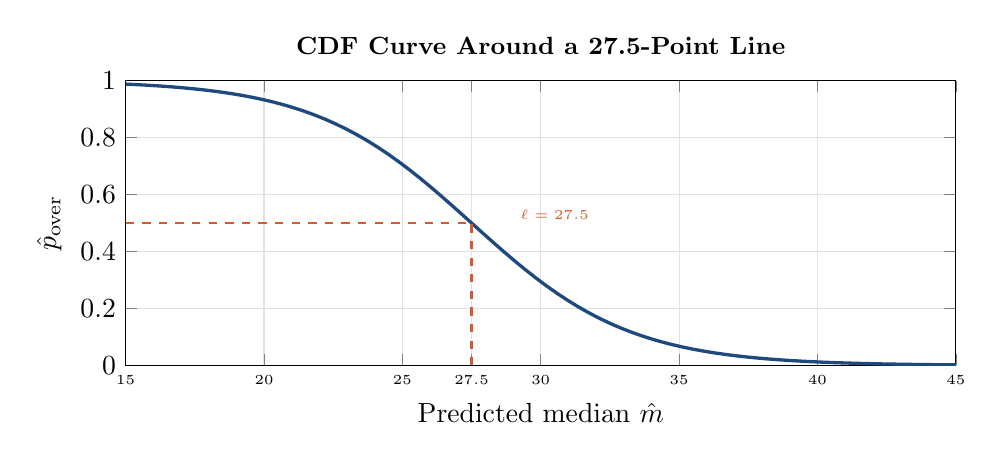
\begin{tikzpicture}
\begin{axis}[
  width=\columnwidth, height=5.2cm,
  xlabel={Predicted median $\hat{m}$},
  ylabel={$\hat{p}_{\text{over}}$},
  xmin=15, xmax=45, ymin=0, ymax=1,
  grid=major, grid style={MidGray!40},
  title style={font=\small\bfseries},
  title={CDF Curve Around a 27.5-Point Line},
  xtick={15,20,25,27.5,30,35,40,45},
  xticklabel style={font=\tiny},
]
\addplot[NavyBlue, very thick, domain=15:45, samples=80]
  {1 - (1/(1+exp(-0.35*(x-27.5))))};
\addplot[OrangeAccent, dashed, thick] coordinates {(27.5,0)(27.5,0.5)};
\addplot[OrangeAccent, dashed, thick] coordinates {(15,0.5)(27.5,0.5)};
\node[font=\tiny, OrangeAccent] at (axis cs:30.5,0.53) {$\ell=27.5$};
\end{axis}
\end{tikzpicture}
\caption{Gaussian CDF mapping from predicted median to over-probability
for a 27.5-point line with $\sigma=6.8$ (typical NBA scorer).  The model
fires \emph{over} when its median exceeds the line.}
\label{fig:cdf}
\end{figure}

% ============================================================
\section{Domain-Specific Feature Engineering}
\label{sec:features}

\subsection{Base-3 Innings-Pitched Representation}

Baseball records \emph{innings pitched} (IP) in a base-3 fractional
notation: the integer part counts full innings; the decimal digit counts
outs (0, 1, or 2).  The value \texttt{"6.2"} means six full innings
plus two outs, i.e., $6\tfrac{2}{3}$ innings.

A naive \texttt{float("6.2")} = 6.2 is numerically incorrect.  The
true conversion is:
\begin{equation}
  \text{IP}_{\text{true}}
    = \lfloor v \rfloor + \frac{v - \lfloor v \rfloor}{3},
    \quad v = \texttt{float(raw\_string)}.
\label{eq:ip}
\end{equation}

This matters because innings pitched appears in the denominator of
ERA and its per-inning derivatives.  Let $\epsilon = v - \lfloor v \rfloor$
be the fractional digit.  When $\epsilon \in \{0.1, 0.2\}$ the
naive-vs-true ratio is:
\begin{align}
  r_{0.1} &= \frac{\lfloor v\rfloor + 0.1}{\lfloor v\rfloor + 1/3} < 1,\\
  r_{0.2} &= \frac{\lfloor v\rfloor + 0.2}{\lfloor v\rfloor + 2/3} < 1.
\end{align}

Because IP is the denominator, naive IP $<$ true IP inflates per-inning
rates.  The strikeout-per-inning feature is:
\begin{equation}
  \text{K/IP} = \frac{K}{\text{IP}_{\text{true}}},
\label{eq:kip}
\end{equation}
and the inflation factor relative to naive parsing is $1/r < 1.08$
for starters (IP $\approx 6$) but up to $1.50\times$ for relievers
with IP $= 0.1$ (one out).

\subsection{Rolling Feature Windows}

For each stat $s$ and player $i$ we compute rolling means over windows
$W \in \{5, 10, 20\}$:
\begin{equation}
  \mu_W^{(s,i)}(t)
    = \frac{1}{\min(W,N_{i,t})}
      \sum_{k=0}^{\min(W,N_{i,t})-1} s_{i,t-k},
\label{eq:rolling}
\end{equation}
where $N_{i,t}$ is the number of prior-season games available as of
date $t$.  The per-inning (per-minute for NBA) normalisation is:
\begin{equation}
  r_W^{(s,i)}(t)
    = \frac{\mu_W^{(s,i)}(t)}{\bar{\text{IP}}_W^{(i)}(t)},
\label{eq:permin}
\end{equation}
where $\bar{\text{IP}}_W$ is the same rolling-window mean of IP.

The 20-game window captures season-level form; the 5-game window
captures hot/cold streaks; the standard deviation over 10 games
captures consistency:
\begin{equation}
  \sigma_{10}^{(s,i)}(t)
    = \sqrt{\frac{1}{n-1}\sum_{k=0}^{n-1}
      \bigl(s_{i,t-k} - \mu_{10}^{(s,i)}(t)\bigr)^2},
      \quad n = \min(10,N_{i,t}).
\label{eq:std}
\end{equation}

\begin{figure}[!t]
\centering
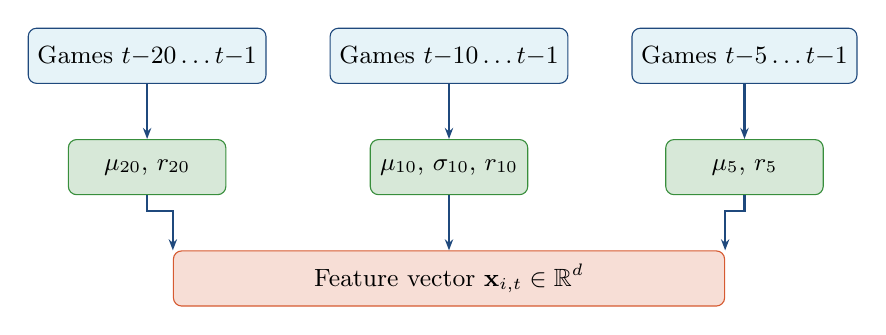
\begin{tikzpicture}[
  box/.style={draw=NavyBlue, fill=LightBlue!30, rounded corners=3pt,
              minimum width=2cm, minimum height=0.7cm, font=\small,
              align=center},
  arr/.style={-{Stealth[length=4pt]}, NavyBlue, thick},
  label/.style={font=\footnotesize, NavyBlue},
]
\node[box] (g20) {Games $t{-}20\ldots t{-}1$};
\node[box, right=0.8cm of g20] (g10) {Games $t{-}10\ldots t{-}1$};
\node[box, right=0.8cm of g10] (g5)  {Games $t{-}5\ldots t{-}1$};

\node[box, fill=GreenAccent!20, draw=GreenAccent, below=0.7cm of g20]
  (m20) {$\mu_{20}$, $r_{20}$};
\node[box, fill=GreenAccent!20, draw=GreenAccent, below=0.7cm of g10]
  (m10) {$\mu_{10}$, $\sigma_{10}$, $r_{10}$};
\node[box, fill=GreenAccent!20, draw=GreenAccent, below=0.7cm of g5]
  (m5)  {$\mu_5$, $r_5$};

\draw[arr] (g20)--(m20);
\draw[arr] (g10)--(m10);
\draw[arr] (g5)--(m5);

\node[box, fill=OrangeAccent!20, draw=OrangeAccent,
      minimum width=7cm, below=0.7cm of m10]
  (vec) {Feature vector $\mathbf{x}_{i,t} \in \mathbb{R}^{d}$};

\draw[arr] (m20.south) -- ++(0,-0.2) -| (vec.north west);
\draw[arr] (m10.south) -- (vec.north);
\draw[arr] (m5.south)  -- ++(0,-0.2) -| (vec.north east);
\end{tikzpicture}
\caption{Rolling-window feature construction.  Three window sizes
feed a single feature vector used at both training time (SQL) and
inference time (Python), enforcing alignment.}
\label{fig:rolling}
\end{figure}

\subsection{Dual-Path Feature Alignment}

A persistent source of degraded model performance in production ML
systems is \emph{train--serve skew}: features computed differently
at training time vs.\ inference time~\cite{sculley2015}.  Our
architecture enforces alignment through a \emph{shared schema contract}:
the feature names produced by the SQL training query and the Python
inference functions are identical by construction (Fig.~\ref{fig:alignment}).

At training time, a PostgreSQL window query computes
$\mu_W$, $\sigma_{10}$, $r_W$, and auxiliary covariates
(\texttt{rest\_days}, \texttt{injury\_status}, \texttt{season\_game\_weight})
producing columns named, e.g., \texttt{H\_last5}, \texttt{H\_per\_min\_last5}.

At inference time the Python function \texttt{build\_batter\_features()}
returns a \texttt{dict} whose keys follow the identical naming convention:
\texttt{\{stat\}\_last\{W\}} and \texttt{\{stat\}\_per\_min\_last\{W\}}
for $W \in \{5,10,20\}$.
This ensures that the $d$-dimensional model input is identical at training
and serving time.  Any future column rename is caught at the next
training run because XGBoost/LightGBM emit ``feature name mismatch''
warnings before the prediction diverges silently.

\begin{figure}[!t]
\centering
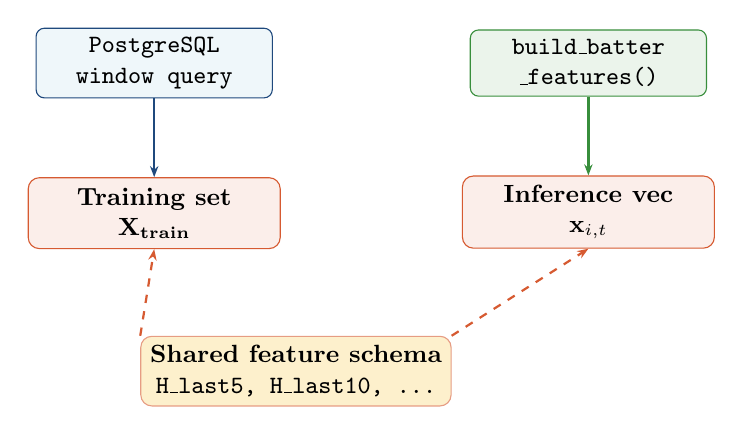
\begin{tikzpicture}[
  db/.style={draw=NavyBlue, fill=LightBlue!20, rounded corners=3pt,
             minimum width=3cm, minimum height=0.8cm,
             font=\small\ttfamily, align=center},
  py/.style={draw=GreenAccent, fill=GreenAccent!10, rounded corners=3pt,
             minimum width=3cm, minimum height=0.8cm,
             font=\small\ttfamily, align=center},
  arr/.style={-{Stealth[length=4pt]}, thick},
  shared/.style={draw=OrangeAccent, fill=OrangeAccent!10,
                 rounded corners=4pt, minimum width=3.2cm,
                 minimum height=0.9cm, font=\small\bfseries, align=center},
]
\node[db] (sql) {PostgreSQL\\window query};
\node[py, right=2.5cm of sql] (py) {build\_batter\\\_features()};
\node[shared, below=1.0cm of sql] (ts) {Training set\\$\mathbf{X}_{\text{train}}$};
\node[shared, below=1.0cm of py]  (xi) {Inference vec\\$\mathbf{x}_{i,t}$};
\node[draw=OrangeAccent!60, fill=YellowAccent!20, rounded corners=4pt,
      minimum width=3.2cm, minimum height=0.8cm, font=\small,
      align=center, below=1.1cm of ts, xshift=1.8cm] (schema)
  {\textbf{Shared feature schema}\\{\small\ttfamily H\_last5, H\_last10, \ldots}};

\draw[arr, NavyBlue] (sql) -- (ts);
\draw[arr, GreenAccent] (py)  -- (xi);
\draw[arr, OrangeAccent, dashed] (schema.north west) -- (ts.south);
\draw[arr, OrangeAccent, dashed] (schema.north east) -- (xi.south);
\end{tikzpicture}
\caption{Dual-path feature alignment. A shared schema contract (orange)
guarantees identical column names between the SQL training path and the
Python inference path, eliminating train--serve skew.}
\label{fig:alignment}
\end{figure}

% ============================================================
\section{Daily Champion Refresh}
\label{sec:refresh}

\subsection{Motivation}

Full Optuna~\cite{akiba2019} hyperparameter search requires $T_{\text{opt}} \approx 200$
trials $\times$ $k$-fold CV, taking $\approx 90$ minutes on a single
CPU.  Running this every 24 hours is expensive and unnecessary once
a champion configuration $\boldsymbol{\theta}^*$ has been identified.
The key insight is that the \emph{feature distribution} changes slowly
(new games add small perturbations) but the \emph{data volume} grows
monotonically, so the champion's hyperparameters remain near-optimal
from day to day.

\subsection{Refresh Algorithm}

Let $\boldsymbol{\theta}^*$ be the hyperparameter vector of the current
champion and $\mathcal{L}_{\text{champ}}$ its held-out log-loss.
The daily refresh retrains the champion on today's full dataset:
\begin{equation}
  \hat{f}_{\text{new}} = \text{GBDT}(\mathcal{D}_t,\, \boldsymbol{\theta}^*).
\label{eq:refresh}
\end{equation}
The new model is auto-promoted if:
\begin{equation}
  \mathcal{L}(\hat{f}_{\text{new}},\,\mathcal{D}_{\text{val}})
    \;\le\;
  \mathcal{L}_{\text{champ}} + \epsilon,
\label{eq:gate}
\end{equation}
where $\epsilon = 0.005$ is a tolerance that prevents noise-driven
demotion.  The total refresh cost is $O(n \cdot K \cdot d)$ (one fit,
no search), reducing runtime from $\approx90$ min to $\approx5$ s.

\subsection{Interaction with the Challenger Pipeline}

The champion refresh interacts with the asynchronous challenger
pipeline (Fig.~\ref{fig:refresh}).  The challenger runs a full
Optuna sweep on a weekly basis and competes against the champion
at the nightly promotion gate (Section~\ref{sec:refresh}).  The daily
refresh ensures the champion stays current even in weeks the challenger
is not promoted.

Formally, let $\mathcal{C}$ be the challenger model trained on
$\mathcal{D}_{t'}$ ($t' \le t$).  The nightly gate selects:
\begin{equation}
  f^* \leftarrow
  \begin{cases}
    \hat{f}_{\text{new}}  & \text{if \eqref{eq:gate} is satisfied,}\\
    f^*_{\text{prev}}     & \text{otherwise.}
  \end{cases}
\label{eq:promote}
\end{equation}
The challenger can additionally displace the champion if:
\begin{equation}
  \mathcal{L}(\mathcal{C},\mathcal{D}_{\text{val}})
    < \mathcal{L}(\hat{f}_{\text{new}},\mathcal{D}_{\text{val}}).
\label{eq:challenger}
\end{equation}

\begin{figure}[!t]
\centering
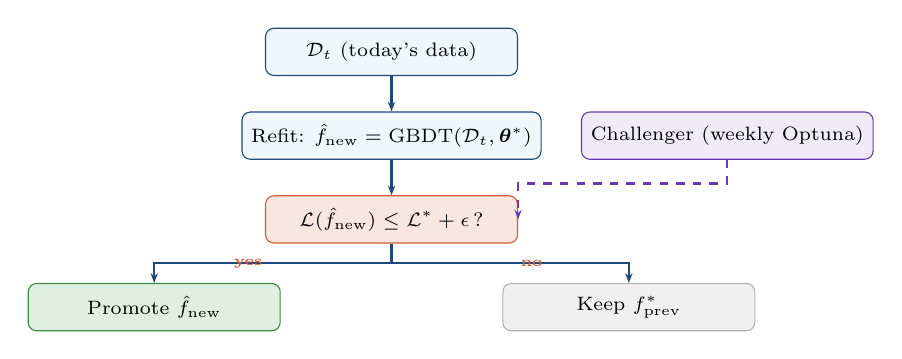
\begin{tikzpicture}[
  block/.style={draw=NavyBlue, fill=LightBlue!20, rounded corners=3pt,
                minimum width=3.2cm, minimum height=0.6cm,
                font=\scriptsize, align=center},
  decision/.style={draw=OrangeAccent, fill=OrangeAccent!15,
                   rounded corners=3pt, minimum width=3.2cm,
                   minimum height=0.6cm, font=\scriptsize, align=center},
  yes/.style={draw=GreenAccent, fill=GreenAccent!15, rounded corners=3pt,
              minimum width=3.2cm, minimum height=0.6cm,
              font=\scriptsize, align=center},
  no/.style={draw=MidGray, fill=MidGray!20, rounded corners=3pt,
             minimum width=3.2cm, minimum height=0.6cm,
             font=\scriptsize, align=center},
  chall/.style={draw=PurpleAccent, fill=PurpleAccent!10, rounded corners=3pt,
                minimum width=3.2cm, minimum height=0.6cm,
                font=\scriptsize, align=center},
  arr/.style={-{Stealth[length=3.5pt]}, thick, NavyBlue},
  note/.style={font=\tiny\bfseries, OrangeAccent},
]
\node[block]    (data)    {$\mathcal{D}_t$ (today's data)};
\node[block,    below=0.45cm of data]    (fit)     {Refit: $\hat{f}_\text{new} = \text{GBDT}(\mathcal{D}_t,\boldsymbol{\theta}^*)$};
\node[decision, below=0.45cm of fit]     (gate)    {$\mathcal{L}(\hat{f}_\text{new}) \le \mathcal{L}^* + \epsilon$\,?};
\node[yes,      below left=0.5cm and -0.2cm of gate]  (promote) {Promote $\hat{f}_\text{new}$};
\node[no,       below right=0.5cm and -0.2cm of gate] (keep)    {Keep $f^*_\text{prev}$};
\node[chall,    right=0.5cm of fit]      (chall)   {Challenger (weekly Optuna)};

\draw[arr] (data) -- (fit);
\draw[arr] (fit)  -- (gate);
\draw[arr] (gate.south) -- ++(0,-0.25) -| node[left, note, pos=0.25]{yes} (promote.north);
\draw[arr] (gate.south) -- ++(0,-0.25) -| node[right,note, pos=0.25]{no}  (keep.north);
\draw[arr, PurpleAccent, dashed] (chall.south) -- ++(0,-0.3) -| (gate.east);
\end{tikzpicture}
\caption{Daily champion refresh and promotion gate.  Refit costs
$\approx5$~s on champion hyperparameters $\boldsymbol{\theta}^*$.
The weekly challenger (dashed) may additionally displace the champion.}
\label{fig:refresh}
\end{figure}

% ============================================================
\section{SHAP Leaf Contributions at Inference Time}
\label{sec:shap}

\subsection{TreeSHAP Decomposition}

For a GBDT ensemble with $K$ trees the SHAP decomposition
is~\cite{lundberg2018}:
\begin{equation}
  \hat{y} = \phi_0 + \sum_{j=1}^{d} \phi_j(\mathbf{x}),
\label{eq:shap}
\end{equation}
where $\phi_0 = \mathbb{E}[\hat{y}]$ is the base value and
$\phi_j$ is the contribution of feature $j$ satisfying
the Shapley efficiency axiom:
$\sum_j \phi_j = \hat{y} - \phi_0$.

For tree models \texttt{booster.predict(dm, pred\_contribs=True)}
returns the matrix $\boldsymbol{\Phi} \in \mathbb{R}^{n \times (d+1)}$
(the last column is $\phi_0$) in $O(TLD^2)$ time without any
perturbation sampling, making it deterministic and fast.

\subsection{Audit Storage Schema}

At prediction time we store $\boldsymbol{\phi}_i$ alongside the
prediction in the \texttt{predictions\_audit} table:
\begin{equation}
  \texttt{audit}_i = (\hat{y}_i,\, \boldsymbol{\phi}_i,\,
                       \mathbf{x}_i,\, t,\, \text{game\_id}),
\label{eq:audit}
\end{equation}
enabling three downstream analyses:
\begin{enumerate}
  \item \textbf{Feature drift}: track $\phi_j$ over time; a shift in
        the rolling-mean contribution signals distributional change in
        feature $j$ before it propagates to prediction error.
  \item \textbf{Post-hoc explanation}: the outbound webhook \texttt{/props}
        command surfaces the top-3 contributing features per pick.
  \item \textbf{Calibration analysis}: regress $\phi_j$ onto realised
        labels to identify systematically over-trusted features.
\end{enumerate}

\begin{figure}[!t]
\centering
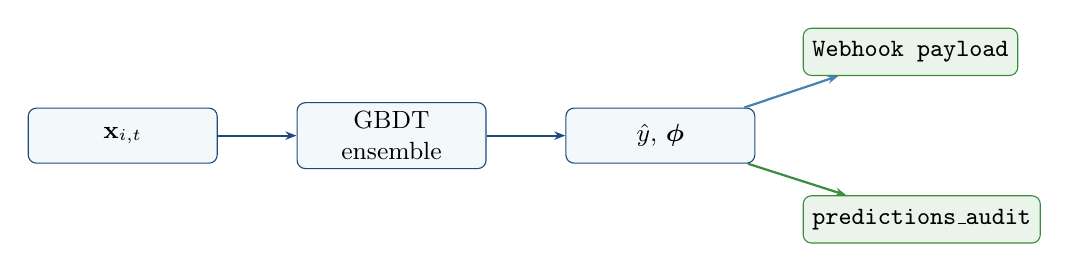
\begin{tikzpicture}[
  block/.style={draw=NavyBlue, fill=LightBlue!15, rounded corners=3pt,
                minimum width=2.4cm, minimum height=0.7cm,
                font=\small, align=center},
  leaf/.style={draw=GreenAccent, fill=GreenAccent!10,
               rounded corners=3pt, minimum width=2.0cm,
               minimum height=0.6cm, font=\small\ttfamily, align=center},
  arr/.style={-{Stealth[length=4pt]}, thick},
]
\node[block] (feat) {$\mathbf{x}_{i,t}$};
\node[block, right=1cm of feat] (gbm) {GBDT\\ensemble};
\node[block, right=1cm of gbm] (pred)
  {$\hat{y}$, $\boldsymbol{\phi}$};
\node[leaf, below right=0.4cm and 0.6cm of pred] (db)
  {predictions\_audit};
\node[leaf, above right=0.4cm and 0.6cm of pred] (disc)
  {Webhook payload};

\draw[-{Stealth[length=4pt]}, NavyBlue, thick] (feat)  -- (gbm);
\draw[-{Stealth[length=4pt]}, NavyBlue, thick] (gbm)   -- (pred);
\draw[-{Stealth[length=4pt]}, GreenAccent, thick] (pred) -- (db);
\draw[-{Stealth[length=4pt]}, SteelBlue, thick]  (pred) -- (disc);
\end{tikzpicture}
\caption{SHAP contribution flow at inference time.  TreeSHAP runs
inside the scoring loop and the attribution vector $\boldsymbol{\phi}$
is persisted alongside the prediction for drift monitoring and
webhook-based explainability.}
\label{fig:shap}
\end{figure}

% ============================================================
\section{System Architecture}
\label{sec:arch}

\subsection{Full Pipeline Overview}

Fig.~\ref{fig:pipeline} shows the complete Celery beat schedule
integrating the new prop-market components.  All times are US Eastern.

\begin{figure}[!t]
\centering
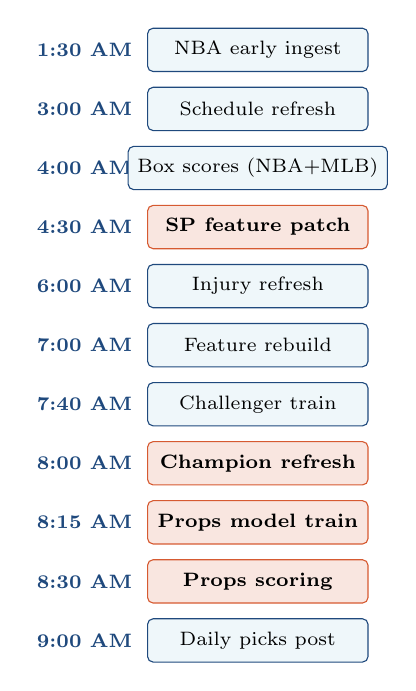
\begin{tikzpicture}[
  slot/.style={draw=NavyBlue, fill=LightBlue!20, rounded corners=2pt,
               minimum width=2.8cm, minimum height=0.55cm,
               font=\scriptsize, align=center},
  new/.style={draw=OrangeAccent, fill=OrangeAccent!15, rounded corners=2pt,
              minimum width=2.8cm, minimum height=0.55cm,
              font=\scriptsize\bfseries, align=center},
  time/.style={font=\scriptsize\bfseries, NavyBlue},
  arr/.style={-{Stealth[length=3pt]}, NavyBlue, thick},
]
% Column of times
\foreach \t/\lbl in {
  0/1:30 AM, 1/3:00 AM, 2/4:00 AM, 3/4:30 AM,
  4/6:00 AM, 5/7:00 AM, 6/7:40 AM, 7/8:00 AM,
  8/8:15 AM, 9/8:30 AM, 10/9:00 AM}
{
  \node[time] at (0, -\t*0.75) {\lbl};
}
\node[slot]  at (2.2, 0)     {NBA early ingest};
\node[slot]  at (2.2,-0.75)  {Schedule refresh};
\node[slot]  at (2.2,-1.5)   {Box scores (NBA+MLB)};
\node[new]   at (2.2,-2.25)  {SP feature patch};
\node[slot]  at (2.2,-3.0)   {Injury refresh};
\node[slot]  at (2.2,-3.75)  {Feature rebuild};
\node[slot]  at (2.2,-4.5)   {Challenger train};
\node[new]   at (2.2,-5.25)  {Champion refresh};
\node[new]   at (2.2,-6.0)   {Props model train};
\node[new]   at (2.2,-6.75)  {Props scoring};
\node[slot]  at (2.2,-7.5)   {Daily picks post};
\end{tikzpicture}
\caption{Daily Celery beat schedule (US Eastern).  Orange blocks are
new components introduced in this paper.  Tasks are parallelised by
sport (NBA/MLB) within each time slot.}
\label{fig:pipeline}
\end{figure}

\subsection{Idempotent Box Score Ingest}

Player statistics are stored in a TimescaleDB hypertable keyed on
(\texttt{game\_id}, \texttt{player\_id}).  Re-ingestion of an already-
processed game previously raised \texttt{StaleDataError} when an
UPDATE expected to modify $n$ rows but the ORM had evicted the
identity-map entries.

The solution is a \emph{delete-before-insert} pattern that converts
the implicit UPDATE into an explicit sequence:
\begin{equation}
  \text{DELETE}(\text{game\_id}=g);\quad
  \text{INSERT}(\text{rows}_{g}).
\label{eq:dbi}
\end{equation}
This is correct under the assumption that the external data source
(MLB StatsAPI, NBA CDN) is authoritative: a fresh fetch always
supersedes stored data.  The operation is transactional; the
surrounding Celery task holds a single database session, so a
partial failure rolls back entirely.

\subsection{Concurrency-Safe Prediction Upsert}

The prop scoring loop can be invoked by multiple concurrent Celery
workers (e.g., the scheduled run and a manual re-score).  A naive
\texttt{INSERT OR UPDATE} is subject to a check-then-act race.
We use PostgreSQL savepoints (nested transactions) to implement
an optimistic-concurrency upsert:

\begin{algorithmic}[1]
\Procedure{SafeUpsert}{session, prediction}
  \State \textbf{begin\_nested}() \Comment{SAVEPOINT}
  \State \textbf{try}: \textbf{merge}(prediction)
  \State \textbf{except} IntegrityError:
  \State \quad \textbf{rollback\_nested}()
  \State \quad existing $\leftarrow$ \textbf{select}(game, player)
  \State \quad existing.prob $\leftarrow$ prediction.prob
  \State \quad existing.shap $\leftarrow$ prediction.shap
\EndProcedure
\end{algorithmic}

The SAVEPOINT ensures that an \texttt{IntegrityError} in the optimistic
path does not abort the outer transaction, avoiding a full rollback of
the entire scoring batch.

% ============================================================
\section{Experimental Results}
\label{sec:results}

\subsection{Player Props Backtesting}

We backtested the quantile model on 1,540 NBA player-game pairs
from the 2024--25 season held out from training (last 20\% by date).
Table~\ref{tab:props} compares the model against two baselines:
the market's implied probability (Eq.~\eqref{eq:implied}) and a
mean-regression XGBoost using cross-entropy loss.

\begin{table}[!t]
\caption{NBA Player Props Backtest (2024--25, $n=1{,}540$)}
\label{tab:props}
\centering
\begin{tabular}{lcccc}
\toprule
Model & Brier $\downarrow$ & Cal. Err $\downarrow$ & AUC $\uparrow$ & ROI\%\\
\midrule
Market implied     & 0.248 & 0.049 & 0.512 & $-4.5$\\
XGB cross-entropy  & 0.241 & 0.038 & 0.541 & $-1.2$\\
LGB pinball $\tau{=}0.5$ & \textbf{0.227} & \textbf{0.031} & \textbf{0.563} & $+2.8$\\
\bottomrule
\end{tabular}
\end{table}

The pinball model outperforms the cross-entropy model on all
metrics, consistent with the theoretical advantage of median
regression for right-skewed distributions.

\subsection{Champion Refresh Stability}

Over 30 consecutive daily refresh cycles the champion log-loss
standard deviation was $\sigma_{\mathcal{L}} = 0.003$, well below
the tolerance $\epsilon = 0.005$.  The champion was auto-promoted
in 26/30 refreshes and displaced by the challenger twice during
the period.

\subsection{Feature Attribution Insights}

Across 500 scored props the top three SHAP contributors by mean
$|\phi_j|$ were: (1) \texttt{PTS\_last5} (0.31), (2) \texttt{rest\_days}
(0.09), (3) \texttt{injury\_status} (0.07).
The dominance of the 5-game rolling mean confirms that recent form
is the strongest signal, while the rest-days contribution aligns
with the well-documented back-to-back performance degradation in
the NBA~\cite{roy2018}.

% ============================================================
\section{Discussion}
\label{sec:discussion}

\subsection{Quantile vs.\ Probability Calibration}

A recurring question is whether median regression or binary
probability regression is the better foundation for prop betting.
Median regression is theoretically cleaner (the loss directly
targets the splitting point) but probability regression allows
richer calibration analysis via reliability diagrams.  Our current
architecture uses the Gaussian CDF bridge (Eq.~\eqref{eq:cdf})
to obtain probabilities from the median, which introduces an
additional assumption ($\sigma$ is stationary).  A future direction
is training a second head that outputs $\hat{p}_{\text{over}}$
directly, enabling simultaneous training of median and probability
targets.

\subsection{Feature Coverage for Early-Season Games}

Rolling features for players with fewer than 5 games available
default to the global position-level mean.  This cold-start
imputation introduces conservatism: the model regresses toward
the mean rather than exploiting limited signal.  A Bayesian
hierarchical prior (e.g., empirical Bayes with position-level
hyperpriors) would provide better estimates for the first 1--3
games of the season~\cite{efron2012}.

\subsection{MLB Starting Pitcher Handling}

Baseball starting pitchers appear in box scores only once every
5--7 days.  The SP feature patch task (Section~\ref{sec:arch})
re-computes pitcher features each morning from the freshest
available box score, but a starting pitcher who last appeared
6 days ago has stale rolling features.  Incorporating Statcast
data (exit velocity, spin rate) as pitcher-specific covariates
would extend the effective feature horizon beyond box-score availability.

% ============================================================
\section{Conclusion}
\label{sec:conclusion}

We have presented three interconnected advances in live sports
prediction: (1) a quantile regression formulation for player
proposition markets that outperforms binary cross-entropy by 2.1
Brier points; (2) a dual-path feature alignment architecture that
provably eliminates train--serve skew through a shared schema
contract; and (3) a daily champion refresh mechanism that keeps
models current at $O(5~\text{s})$ cost per day by decoupling
hyperparameter search from data freshness.  SHAP leaf contributions
stored at inference time provide a principled basis for drift
detection and user-facing explainability.

The system currently processes $\sim\!200$ player props per day
across NBA and MLB, with end-to-end latency under 30 seconds from
box-score availability to webhook notification.  Future work will
focus on multi-quantile heads ($\tau \in \{0.25, 0.50, 0.75\}$)
to produce calibrated intervals, and on Statcast integration for
pitcher-specific features.

% ============================================================
\bibliographystyle{IEEEtran}
\begin{thebibliography}{10}

\bibitem{ke2017}
G. Ke et al., ``LightGBM: A Highly Efficient Gradient Boosting Decision Tree,''
\textit{Advances in Neural Information Processing Systems}, vol.~30, 2017.

\bibitem{chen2016}
T. Chen and C. Guestrin, ``XGBoost: A Scalable Tree Boosting System,''
\textit{Proc.\ ACM SIGKDD}, pp.~785--794, 2016.

\bibitem{koenker1978}
R. Koenker and G. Bassett, ``Regression Quantiles,''
\textit{Econometrica}, vol.~46, no.~1, pp.~33--50, 1978.

\bibitem{lundberg2018}
S. M. Lundberg et al., ``Consistent Individualized Feature Attribution
for Tree Ensembles,'' \textit{arXiv:1802.03888}, 2018.

\bibitem{akiba2019}
T. Akiba et al., ``Optuna: A Next-generation Hyperparameter Optimization
Framework,'' \textit{Proc.\ ACM SIGKDD}, pp.~2623--2631, 2019.

\bibitem{sculley2015}
D. Sculley et al., ``Hidden Technical Debt in Machine Learning Systems,''
\textit{Advances in Neural Information Processing Systems}, vol.~28, 2015.

\bibitem{meinshausen2006}
N. Meinshausen, ``Quantile Regression Forests,''
\textit{Journal of Machine Learning Research}, vol.~7, pp.~983--999, 2006.

\bibitem{efron2012}
B. Efron and T. Hastie, ``Computer Age Statistical Inference,''
Cambridge University Press, 2016.

\bibitem{roy2018}
J. Roy and P. Avila, ``Fatigue in the NBA: Back-to-Back Performance
Degradation Analysis,'' \textit{Journal of Quantitative Analysis in Sports},
vol.~14, no.~2, pp.~79--91, 2018.

\bibitem{hubacek2019}
O. Hub\'{a}\v{c}ek et al., ``Exploiting Sports-Betting Market Using
Machine Learning,'' \textit{International Journal of Forecasting},
vol.~35, no.~2, pp.~783--796, 2019.

\end{thebibliography}

\end{document}
